\section{Evaluation}

\begin{figure*}[t!]
  \centering
  %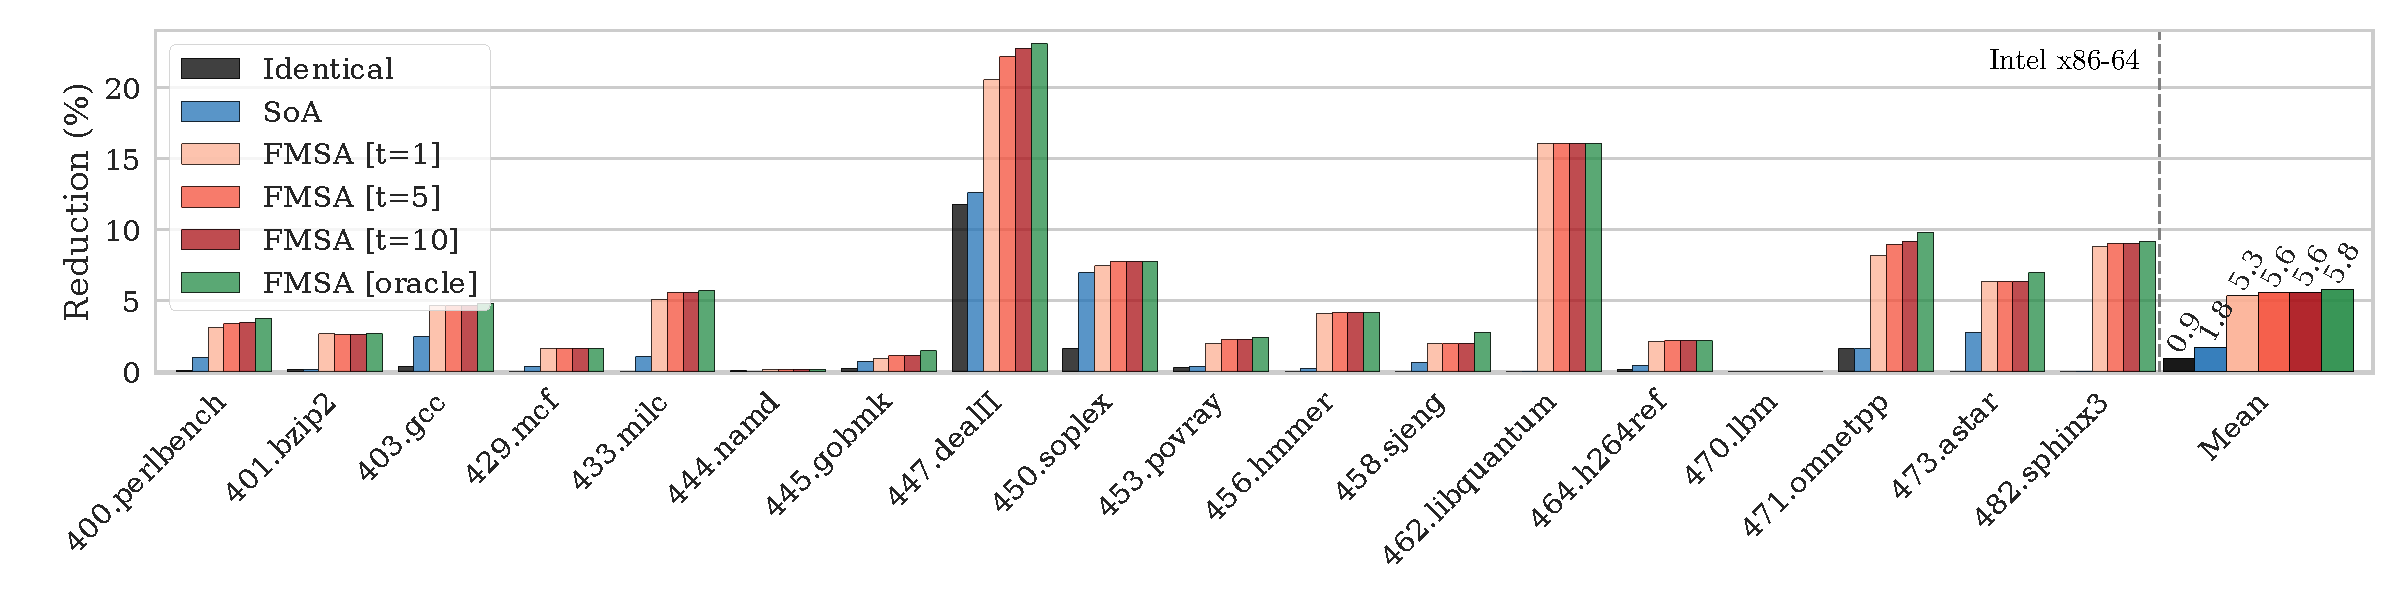
\includegraphics[width=\linewidth]{figs/reduction-obj-intel-label.pdf} \\
  %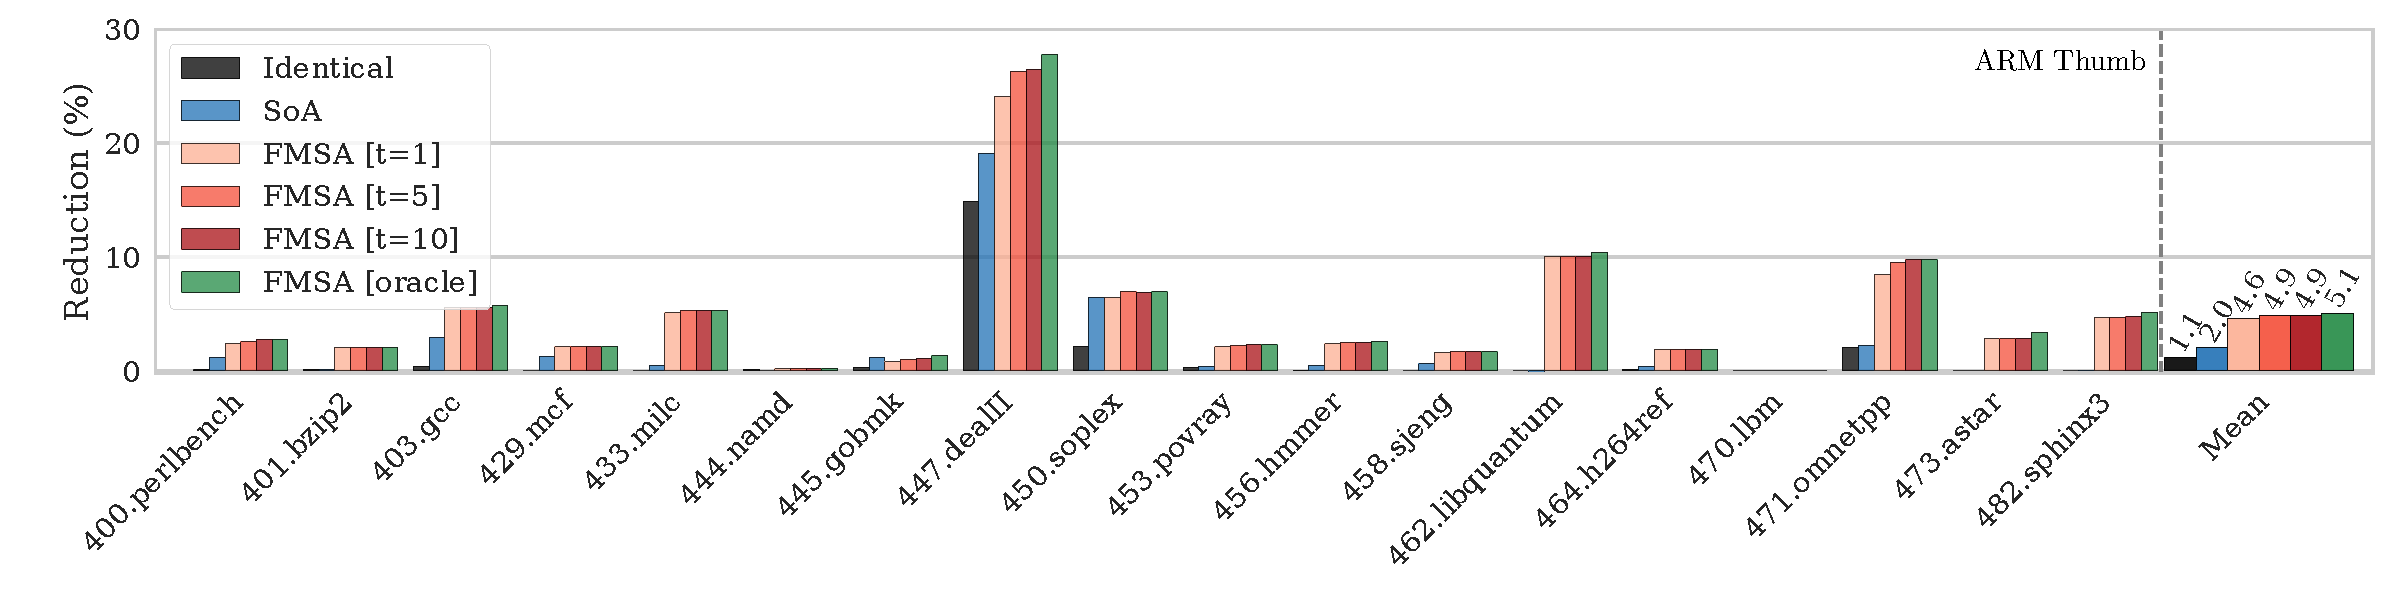
\includegraphics[width=\linewidth]{figs/reduction-obj-arm-label.pdf}
  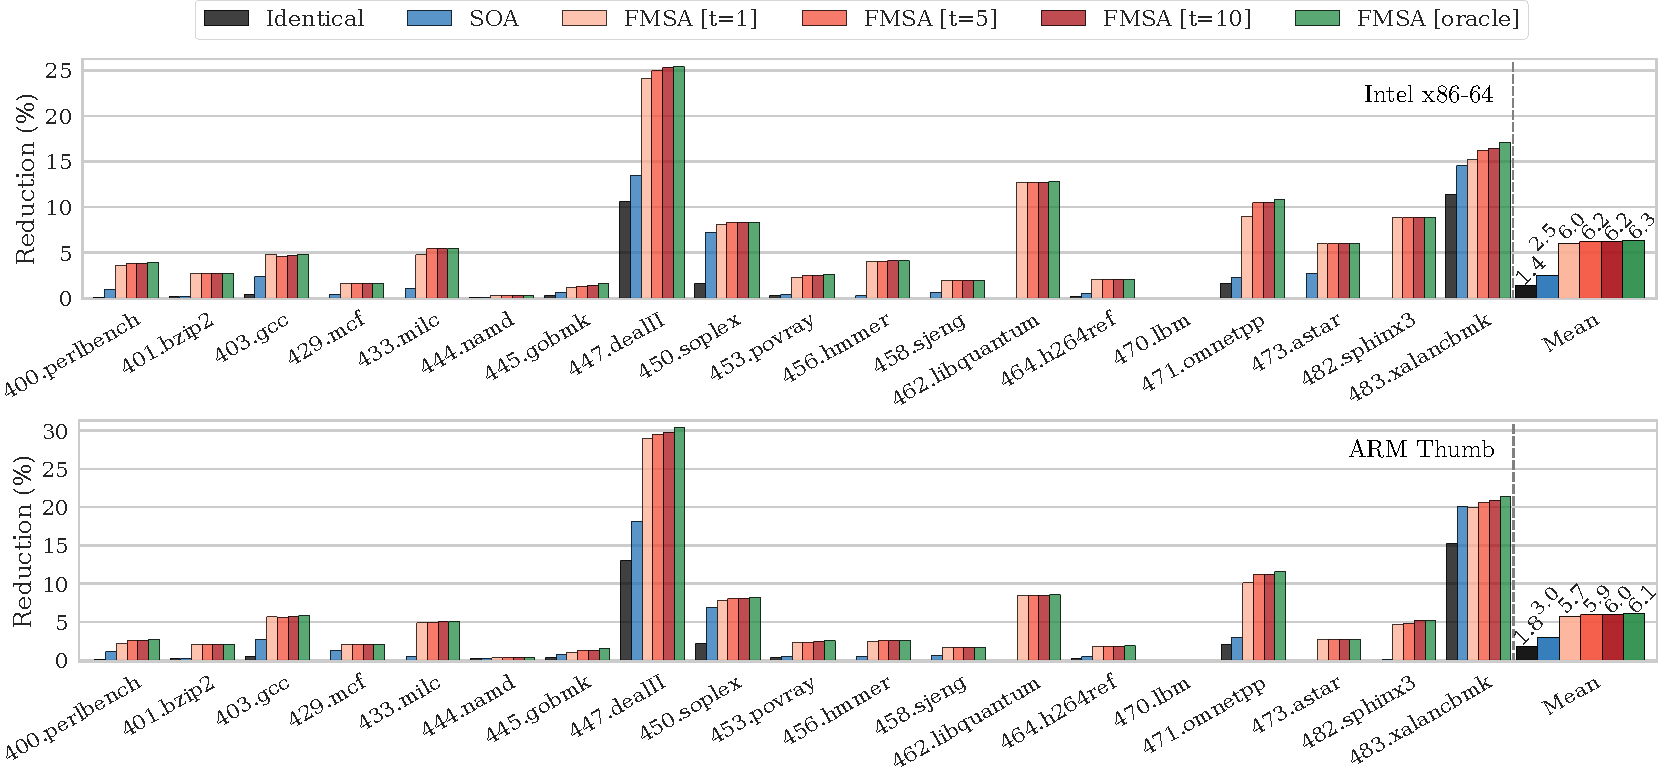
\includegraphics[width=\linewidth]{figs/code-size-reduction-spec.pdf}
	\caption{Object file size reduction for Intel (top) and ARM (bottom). We evaluate our approach (FMSA) under four different exploration thresholds, which
      control how many potential merging pairs we examine for each function before making a decision. Even for a threshold of one, we outperform the state-of-the-art
	  by 2.4$\times$~(Intel) and 1.9$\times$~(ARM).}
  \label{fig:reduction-obj}
\end{figure*}

In this section, we evaluate the proposed optimization, where we analyze our
improvements on code size reduction, as well as its impact on the program's
performance and compilation-time.

\subsection{Experimental Setup}
We compare our optimization against the state-of-the-art~\cite{edler14}
%function merging approach of Edler von Koch et al.~\cite{edler14}
and LLVM's identical~\cite{llvm-fm} function merging techniques. In our evaluation, we refer to identical function merging as \textit{Identical}, the state-of-the-art as \textit{SOA}, and our
approach as \textit{FMSA}.
We also run LLVM's identical function merging before both \textit{SOA} and \textit{FMSA}, as this helps to reduce
compilation time by efficiently reducing the number of trivially mergeable functions.

All optimizations are implemented in LLVM v8 and evaluated on two benchmark suites: the C/C++ SPEC CPU2006~\cite{spec} and MiBench~\cite{mibench01}.
We target two different instruction sets, the Intel x86-64 and the ARM Thumb. Our Intel test bench has a quad-core 3.4~GHz Intel Core i7 CPU with 16~GiB of RAM.
%The operating system is openSUSE 42.2 with Linux kernel version 4.4.27.
The ARM test bench has a Cortex-A53 ARMv8 CPU of 1.4~GHz with 1~GiB of RAM.
%The operating system of the ARM platform is a Raspbian.
We use the Intel platform for compiling for either target. As a result, compilation-time is almost
identical for both targets. Changing the target only affects the behavior of the backend, a very
short part of the pipeline. Because of that, we only report compilation-time overhead results for
one of the targets, the Intel ISA.

For the proposed optimization, we vary the exploration threshold (Section~\ref{sec:framework})
and we present the results for a range of threshold values. We also show the results for the oracle exploration strategy, which
instead of using a rank-based greedy approach, merges a function with all candidates and chooses the best one.
%The oracle represents the results assuming a perfect ranking strategy.
%However, the oracle has a very costly quadratic exploration, as explained in
%Section~\ref{sec:framework}.
This oracle is a perfect ranking strategy but is unrealistic. It requires a very costly quadratic exploration, as explained in
Section~\ref{sec:framework}. \fixme{ZW: I suggest we call ``oracle" exhaustive-exploration instead. ``oracle" is often used to refer the
up-bound performance.}

\subsection{Code-Size Reduction}

Figure~\ref{fig:reduction-obj} reports the code size reduction over the baseline for the linked object. %These results show how much we can improve over the existing techniques, by having a more powerful solution, and how close we
%can get to the oracle with our ranking-based exploration framework.
We observe similar trends of code size reduction on both target architectures. This is expected because the
optimizations are applied at the platform-independent IR level. Changing the target architecture introduces only second order effects,
such as slightly different decisions due to the different cost model (LLVM's TTI) and differences in how the IR is encoded into binary.

Our approach, FMSA, significantly improves over the state-of-the art (SoA). For the Intel platform, FMSA can achieve an average code size
reduction of up to 5.8\% (or 5.3\% with the lowest exploration threshold), while the SoA and Identical had an average reduction of 1.8\% and 0.9\%,
respectively. Similarly, for the ARM platform, FMSA can achieve an average code size reduction of up to 5.1\% (or 4.6\% with the lowest
threshold), while SoA and Identical had an average reduction of 2\% and 1.1\%, respectively. For several of the benchmarks, the
proposed technique achieves impressive code size reduction compared to other merging approaches.

%Table~\ref{tab:reduction} highlights some of these results for both platforms. In two cases, \texttt{462.libquantum} and \texttt{482.sphinx3}, the state-of-the-art slightly
%increases code size, while FMSA reduces size significantly.  The only case where SOA outperforms FMSA is on the \texttt{445.gobmk}
%benchmark on the ARM platform.
%There are little opportunities for function merging on that benchmark and FSMA misses a few of them.
%However, we can easily fix this by increasing the exploration threshold. For exhaustive exploration, FMSA improves over the SoA,
%with a code size reduction of 1.33\%. In all other cases, FMSA is always equal or better than all other function-merging optimizations, usually by a significant margin.

%\begin{table}[]
%\centering
%\scalebox{0.8}{
%\begin{tabular}{lccc}
%\toprule
%\multicolumn{1}{c}{\textbf{Benchmarks}} & \textbf{Identical} & \textbf{SoA}  & \textbf{FMSA {[}t=1{]}} \\
%\midrule
%%%400.perlbench                      & 0.09 / 0.09     & 1.03 / 1.15   & 3.13 / 2.40     \\
%\rowcolor{evencolor} 401.bzip2        & 0.15 / 0.16     & 0.15 / 0.16   & 2.67 / 2.09     \\
%%%403.gcc                            & 0.36 / 0.43     & 2.48 / 2.89   & 4.71 / 5.59     \\
%%%429.mcf                            & 0 / 0           & 0.41 / 1.29    & 1.66 / 2.11    \\
%433.milc                              & 0 / 0           & 1.08 / 0.46   & 5.09 / 5.12     \\
%%%444.namd                           & 0.10 / 0.14     & 0 / 0         & 0.20 / 0.17     \\
%\rowcolor{evencolor} 447.dealII       & 11.77 / 14.83   & 12.59 / 19.12 & 20.57 / 24.08   \\
%445.gobmk                             & 0.26 / 0.32     & 0.77 / 1.15   & 0.96 / 0.78     \\
%%%450.soplex                         & 1.62 / 2.16     & 6.99 / 6.47   & 7.46 / 6.48     \\
%\rowcolor{evencolor} 453.povray       & 0.28 / 0.33     & 0.38 / 0.40   & 2.04 / 2.12     \\
%456.hmmer                             & 0 / 0           & 0.27 / 0.50   & 4.15 / 2.40     \\
%%%458.sjeng                          & 0 / 0           & 0.63 / 0.63   & 1.97 / 1.62     \\
%\rowcolor{evencolor} 462.libquantum   & 0 / 0           & -0.07 / -0.17 & 16.08 / 10.04   \\
%%%464.h264ref                        & 0.16 / 0.14     & 0.47 / 0.40   & 2.16 / 1.86     \\
%%%470.lbm                            & 0 / 0           & 0 / 0         & 0 / 0           \\
%471.omnetpp                           & 1.65 / 2.08     & 1.64 / 2.27   & 8.18 / 8.47     \\
%\rowcolor{evencolor} 473.astar        & 0 / 0           & 2.76 / 0      & 6.33 / 2.81     \\
%482.sphinx3                           & 0 / 0           & -0.06 / 0.06  & 8.85 / 4.72     \\
%\bottomrule
%\end{tabular}
%}
%\caption{Highlights of code reduction results (in percentages) on \textit{Intel / ARM} platforms. }
%\label{tab:reduction}
%\end{table}

In most cases, LLVM's identical function merging has very little impact on code
size.
We see noticeable impact only on some of the C++ benchmarks, namely,
\texttt{447.dealII}, \texttt{450.soplex}, \texttt{471.omnetpp}, \texttt{483.xalancbmk}.
These are the cases that identical function merging was designed to handle,
duplicate functions due to heavy use of templating.
%But even on these benchmarks FMSA outperforms LLVM, with an improvement of
%almost 6$\times$ on \texttt{471.omnetpp}.
Although the state-of-the-art improves over LLVM's identical function merging,
it still gets most of its code size reduction for benchmarks with heavy use of templating.
In addition to achieving better results in all of these cases, our technique
%On the other hand, FMSA is able to achieve better results in all these cases.
%FMSA is designed to merge a superset of the functions that the LLVM identical
%function merging can handle while having much less restrictions than the
%state-of-the-art, so it is able to achieve better results in all these cases.
%Moreover, our technique
also shows remarkable reductions on several of the
C benchmarks, especially \texttt{462.libquantum} and \texttt{482.sphinx3}, where
other techniques have no real impact.


In Section~\ref{sec:motivation}, we show two examples extracted from
\texttt{462.libquantum} and \texttt{482.sphinx3}, where we detail how existing
techniques fail to merge similar functions in these benchmarks.
Our technique is the \textit{first} that can handle these examples, producing
merged functions equivalent to the handwritten ones shown in
Figures~\ref{fig:sphinx-example} and~\ref{fig:libquantum-example}.
%as we overcome major limitations from the existing techniques.
%%TODO: add some statistics about these two benchmarks

%Figure~\ref{fig:libquantum-example} shows an example of two functions\footnote{We
%have changed very lightly some of the names used in the functions so that the
%code fits nicely in the paper. The original names of the functions are:
%quantum\_cond\_phase and quantum\_cond\_phase\_inv.}
%from the 462.libquantum benchmark that are merged by the proposed optimization.
%The proposed function-merging technique is the \textit{first} technique able to
%merge these two functions.
%Although they are very similar functions, the state-of-the-art is unable to
%merge them since their CFGs are not structurally identical.
%For the proposed optimization, however, these two functions receive a similarity
%score above $0.49$, which puts them at the top of the rank, and the
%profitability cost model estimates a code-size reduction of 40\%.
%Overall, our optimization was able to merge nine pairs of functions for the
%462.libquantum benchmark.
%Similar to the example shown, all of them were top ranked based on their
%fingerprint similarity.

%Note that functions that are identical at the IR or machine level are not
%necessarily identical at the source level.
%Figure~\ref{fig:identical-example} shows two real functions extract from the
%447.dealII program in the SPEC CPU2006~\cite{spec} benchmark suite.
%Although these two functions are not identical at the source level, they become
%identical after a template specialization and some optimizations are applied, in
%particular, constant propagation, constant folding, and dead-code elimination.
%Specializing \verb|dim| to $1$ enables to completely remove the loop in the
%function \verb|PolynomialSpace|.
%Similarly, specializing \verb|dim| to $1$ results in only the first iteration
%of the loop in the function \verb|TensorProductPolynomials| being executed.
%The compiler is able to statically analyze and simiplify the loops in both
%functions, resulting in the identical functions shown at the bottom of
%Figure~\ref{fig:identical-example}.


%\begin{figure*}[t]
%  \centering
%  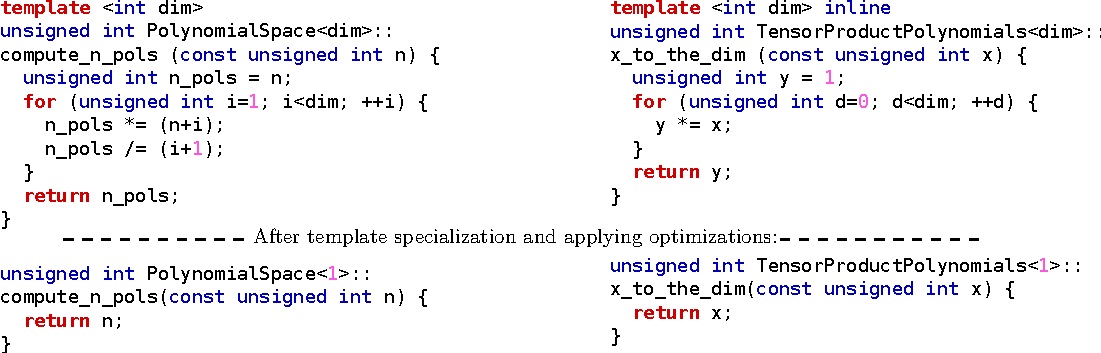
\includegraphics[width=0.95\linewidth]{figs/identical-example.pdf}
%  \caption{Two function extracted from the 447.dealII benchmark that are not
%           identical at the source level, but after applying template
%           specialization and optimizations they become identical at the IR
%           level.}
%  \label{fig:identical-example}
%\end{figure*}



%\begin{table}[h]
%\centering
%\caption{Number and size of functions present in each SPEC CPU2006 benchmark just before function merging, as well as number of merge operations applied by each technique.}
%\scalebox{0.8}{
%\begin{tabular}{llllll}
%\toprule
%\multicolumn{1}{c}{\textbf{Benchmarks}} & \textbf{\#Functions} & \textbf{Min/Avg/Max Size} &\textbf{Identical} & \textbf{SOA}  & \textbf{FMSA {[}t=1{]}} \\
%\midrule
%                     400.perlbench      & 1699   & 1 / 125 / 12501    & 12     & 103   & 175    \\
%\rowcolor{evencolor} 401.bzip2          & 74     & 1 / 206 / 5997     & 0      & 0     & 7      \\
%                     403.gcc            & 4541   & 1 / 127.7 / 20688  & 136    & 341   & 614    \\
%\rowcolor{evencolor} 429.mcf            & 24     & 18 / 87.25 / 297   & 0      & 1     & 1      \\
%                     433.milc           & 235    & 1 / 67.69 / 416    & 0      & 6     & 26     \\
%\rowcolor{evencolor} 444.namd           & 99     & 1 / 570.64 / 1698  & 1      & 1     & 5      \\
%                     445.gobmk          & 2511   & 1 / 43.22 / 3140   & 183    & 485   & 436    \\
%\rowcolor{evencolor} 447.dealII         & 7380   & 1 / 60.63 / 4856   & 1835   & 2785  & 2974   \\
%                     450.soplex         & 1035   & 1 / 73.27 / 1719   & 27     & 125   & 156    \\
%\rowcolor{evencolor} 453.povray         & 1585   & 1 / 98.05 / 5324   & 60     & 112   & 193    \\
%                     456.hmmer          & 487    & 1 / 99.98 / 1511   & 3      & 16    & 45     \\
%\rowcolor{evencolor} 458.sjeng          & 134    & 1 / 145.06 / 1252  & 0      & 5     & 11     \\
%                     462.libquantum     & 95     & 1 / 56.64 / 626    & 0      & 1     & 9      \\
%\rowcolor{evencolor} 464.h264ref        & 523    & 1 / 171.42 / 5445  & 3      & 22    & 50     \\
%                     470.lbm            & 17     & 6 / 123.41 / 680   & 0      & 0     & 0      \\
%\rowcolor{evencolor} 471.omnetpp        & 1406   & 1 / 26.9 / 611     & 45     & 69    & 227    \\
%                     473.astar          & 101    & 1 / 67.11 / 584    & 0      & 2     & 4      \\
%\rowcolor{evencolor} 482.sphinx3        & 326    & 1 / 80 / 924       & 2      & 6     & 24     \\
%                     483.xalancbmk      & 14191  & 1 / 38.58 / 3809   & 3057   & 4573  & 4342   \\
%\bottomrule
%\end{tabular}
%}
%\label{tab:stats}
%\end{table}

\begin{table}[h]
\centering
\caption{Number and size of functions present in each SPEC CPU2006 benchmark just before function merging, as well as number of merge operations applied by each technique.}
\scalebox{0.71}{
\begin{tabular}{lllllll}
\toprule
\multicolumn{1}{c}{\textbf{Benchmarks}} & \textbf{\#Fns} & \textbf{Min/Avg/Max Size} &\textbf{Identical} & \textbf{SOA}  & \textbf{FMSA{[}t=1{]}} & \textbf{FMSA{[}t=10{]}} \\
\midrule
                     400.perlbench      & 1699   & 1 / 125 / 12501    & \small 12     & \small 103   & \small 175  & \small 200  \\
\rowcolor{evencolor} 401.bzip2          & 74     & 1 / 206 / 5997     & \small 0      & \small 0     & \small 7    & \small 7    \\
                     403.gcc            & 4541   & 1 / 127.7 / 20688  & \small 136    & \small 341   & \small 614  & \small 710  \\
\rowcolor{evencolor} 429.mcf            & 24     & 18 / 87.25 / 297   & \small 0      & \small 1     & \small 1    & \small 1    \\
                     433.milc           & 235    & 1 / 67.69 / 416    & \small 0      & \small 6     & \small 26   & \small 34   \\
\rowcolor{evencolor} 444.namd           & 99     & 1 / 570.64 / 1698  & \small 1      & \small 1     & \small 5    & \small 5    \\
                     445.gobmk          & 2511   & 1 / 43.22 / 3140   & \small 183    & \small 485   & \small 436  & \small 605  \\
\rowcolor{evencolor} 447.dealII         & 7380   & 1 / 60.63 / 4856   & \small 1835   & \small 2785  & \small 2974 & \small 3315 \\
                     450.soplex         & 1035   & 1 / 73.27 / 1719   & \small 27     & \small 125   & \small 156  & \small 163  \\
\rowcolor{evencolor} 453.povray         & 1585   & 1 / 98.05 / 5324   & \small 60     & \small 112   & \small 193  & \small 212  \\
                     456.hmmer          & 487    & 1 / 99.98 / 1511   & \small 3      & \small 16    & \small 45   & \small 47   \\
\rowcolor{evencolor} 458.sjeng          & 134    & 1 / 145.06 / 1252  & \small 0      & \small 5     & \small 11   & \small 11   \\
                     462.libquantum     & 95     & 1 / 56.64 / 626    & \small 0      & \small 1     & \small 9    & \small 9    \\
\rowcolor{evencolor} 464.h264ref        & 523    & 1 / 171.42 / 5445  & \small 3      & \small 22    & \small 50   & \small 52   \\
                     470.lbm            & 17     & 6 / 123.41 / 680   & \small 0      & \small 0     & \small 0    & \small 0    \\
\rowcolor{evencolor} 471.omnetpp        & 1406   & 1 / 26.9 / 611     & \small 45     & \small 69    & \small 227  & \small 270  \\
                     473.astar          & 101    & 1 / 67.11 / 584    & \small 0      & \small 2     & \small 4    & \small 4    \\
\rowcolor{evencolor} 482.sphinx3        & 326    & 1 / 80 / 924       & \small 2      & \small 6     & \small 24   & \small 26   \\
                     483.xalancbmk      & 14191  & 1 / 38.58 / 3809   & \small 3057   & \small 4573  & \small 4342 & \small 4887 \\
\bottomrule
\end{tabular}
}
\label{tab:stats}
\end{table}

Table~\ref{tab:stats} provides detailed statistics for the SPEC CPU2006.
We show how many functions (\#Fns) are present in the linked program
just before the merging pass, as well as
the average, minimum, and maximum size of these functions, in number of instructions, at
this same point in the compilation pipeline.
We also report how many pair-wise merge operations are
performed by each one of the function merging techniques.
Note that in almost all cases FMSA performs significantly more merge operations than the other
techniques.
There are only two cases where FMSA with exploration threshold of one finds fewer
profitable merges than the state-of-the-art. This is due to our aggressive pruning
of the search space with our ranking mechanism. Simply increasing the threshold, e.g. to ten,
allows FMSA to merge more functions. In any case, these extra merge operations of the state-of-the-art
have little effect on the overall code size reduction. The state-of-the-art is more likely to fail to
merge large functions and succeed with small ones, so even when merging more functions, it does not
reduce code size as much as FMSA.

\subsubsection*{MiBench: Embedded Benchmark Suite}

We have shown that our technique achieves good results when applied on the SPEC
CPU suite. It reduces size not only on templated C++ benchmarks, like other
techniques, but also on C benchmarks where merging opportunities should
be almost non-existant. Here, we further explore how FMSA handles such
cases by applying it on the MiBench suite, a collection of small C programs
each one composed of a small number of functions. 

Figure~\ref{fig:code-size-reduction-mibench} shows the object file reduction
for the MiBench programs on the Intel platform. Our best result is for the \texttt{rijndael} benchmark,
which implements the well-known AES encryption. FMSA merges the two largest functions, namely,
\texttt{encrypt} and \texttt{decrypt}.
Inspecting the LLVM IR for the \texttt{rijndael} benchmark, we observe that
the two functions contain a total of 2494 instructions, over 70\% of the code.
When we merge them by sequence alignment, we create a single function with
only 1445 instruction, a 42\% reduction in the number of IR instructions. This
translates into a 20.6\% reduction in the linked object file.

\begin{table}[h]
\centering
\caption{Number and size of functions present in each MiBench benchmark just before function merging, as well as number of merge operations applied by each technique.}
\scalebox{0.75}{
\begin{tabular}{lllllll}
\toprule
\multicolumn{1}{c}{\textbf{Benchmarks}} & \textbf{\#Fns} & \textbf{Min/Avg/Max Size} &\textbf{Identical} & \textbf{SOA}  & \textbf{FMSA{[}t=1{]}}  & \textbf{FMSA{[}t=10{]}} \\
\midrule
                     CRC32         & 4     & 8 / 24.75 / 39       & \small 0     & \small 0   & \small 0    & \small 0   \\
\rowcolor{evencolor} FFT           & 7     & 7 / 49.86 / 144      & \small 0     & \small 0   & \small 0    & \small 0   \\
                     adpcm\_c      & 3     & 37 / 73 / 100        & \small 0     & \small 0   & \small 0    & \small 0   \\
\rowcolor{evencolor} adpcm\_d      & 3     & 37 / 73 / 100        & \small 0     & \small 0   & \small 0    & \small 0   \\
                     basicmath     & 5     & 4 / 70.8 / 232       & \small 0     & \small 0   & \small 0    & \small 0   \\
\rowcolor{evencolor} bitcount      & 19    & 4 / 22.26 / 63       & \small 0     & \small 1   & \small 3    & \small 3   \\
                     blowfish\_d   & 8     & 1 / 245.38 / 824     & \small 0     & \small 0   & \small 0    & \small 0   \\
\rowcolor{evencolor} blowfish\_e   & 8     & 1 / 245.38 / 824     & \small 0     & \small 0   & \small 0    & \small 0   \\
                     jpeg\_c       & 322   & 1 / 100.52 / 1269    & \small 2     & \small 6   & \small 8    & \small 11  \\
\rowcolor{evencolor} jpeg\_d       & 310   & 1 / 98.93 / 1269     & \small 3     & \small 6   & \small 10   & \small 10  \\
                     dijkstra      & 6     & 2 / 33 / 89          & \small 0     & \small 0   & \small 0    & \small 0   \\
\rowcolor{evencolor} ghostscript   & 3446  & 1 / 54.2 / 4218      & \small 53    & \small 53  & \small 234  & \small 250 \\
                     gsm           & 69    & 1 / 97.06 / 737      & \small 0     & \small 3   & \small 8    & \small 8   \\
\rowcolor{evencolor} ispell        & 84    & 1 / 105.51 / 1082    & \small 0     & \small 2   & \small 5    & \small 5   \\
                     patricia      & 5     & 1 / 77 / 167         & \small 0     & \small 0   & \small 0    & \small 0   \\
\rowcolor{evencolor} pgp           & 310   & 1 / 88.52 / 1845     & \small 0     & \small 1   & \small 10   & \small 10  \\
                     qsort         & 2     & 11 / 50 / 89         & \small 0     & \small 0   & \small 0    & \small 0   \\
\rowcolor{evencolor} rijndael      & 7     & 46 / 472.29 / 1247   & \small 0     & \small 0   & \small 1    & \small 1   \\
                     rsynth        & 46    & 1 / 97.28 / 778      & \small 0     & \small 0   & \small 0    & \small 0   \\
\rowcolor{evencolor} sha           & 7     & 12 / 53.29 / 150     & \small 0     & \small 0   & \small 0    & \small 0   \\
                     stringsearch  & 10    & 3 / 47.9 / 99        & \small 0     & \small 0   & \small 1    & \small 1   \\
\rowcolor{evencolor} susan         & 19    & 15 / 291.84 / 1212   & \small 0     & \small 0   & \small 1    & \small 1   \\
                     typeset       & 362   & 1 / 354.47 / 12125   & \small 1     & \small 4   & \small 31   & \small 35  \\
\bottomrule
\end{tabular}
}
\label{tab:stats-mibench}
\end{table}


\begin{figure*}[t]
  \centering
  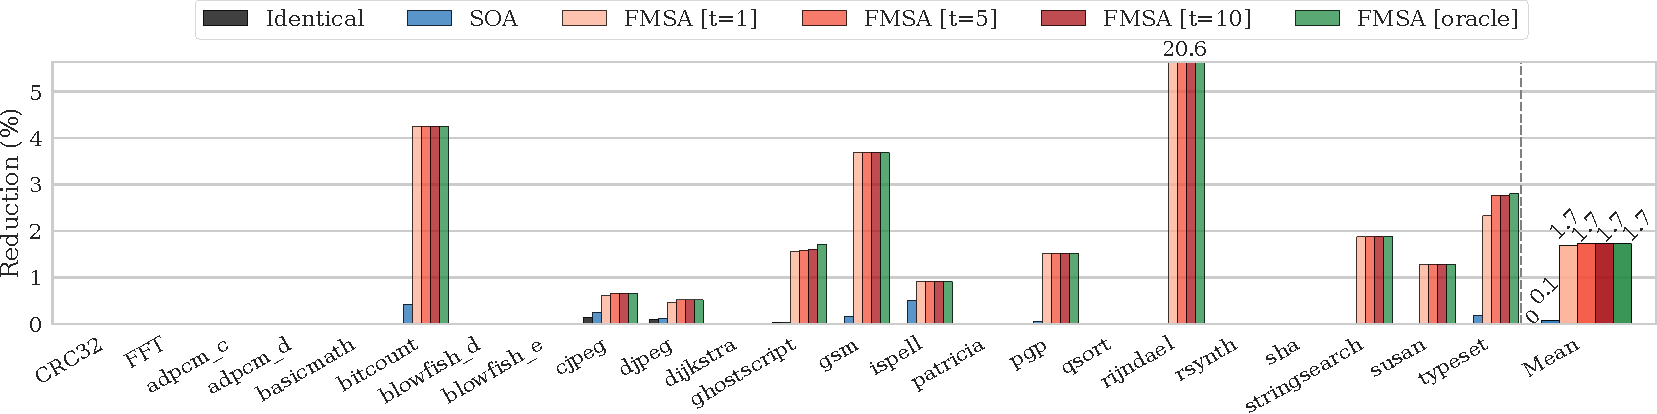
\includegraphics[width=\linewidth]{figs/code-size-reduction-mibench.pdf}
  \caption{Object file size reduction for Intel on the Mibench benchmark suite.
   Our approach (FMSA) is the only one able to achieve a meaningful reduction on these benchmarks.}
  \label{fig:code-size-reduction-mibench}
\end{figure*}

\begin{figure*}[t]
  \centering
  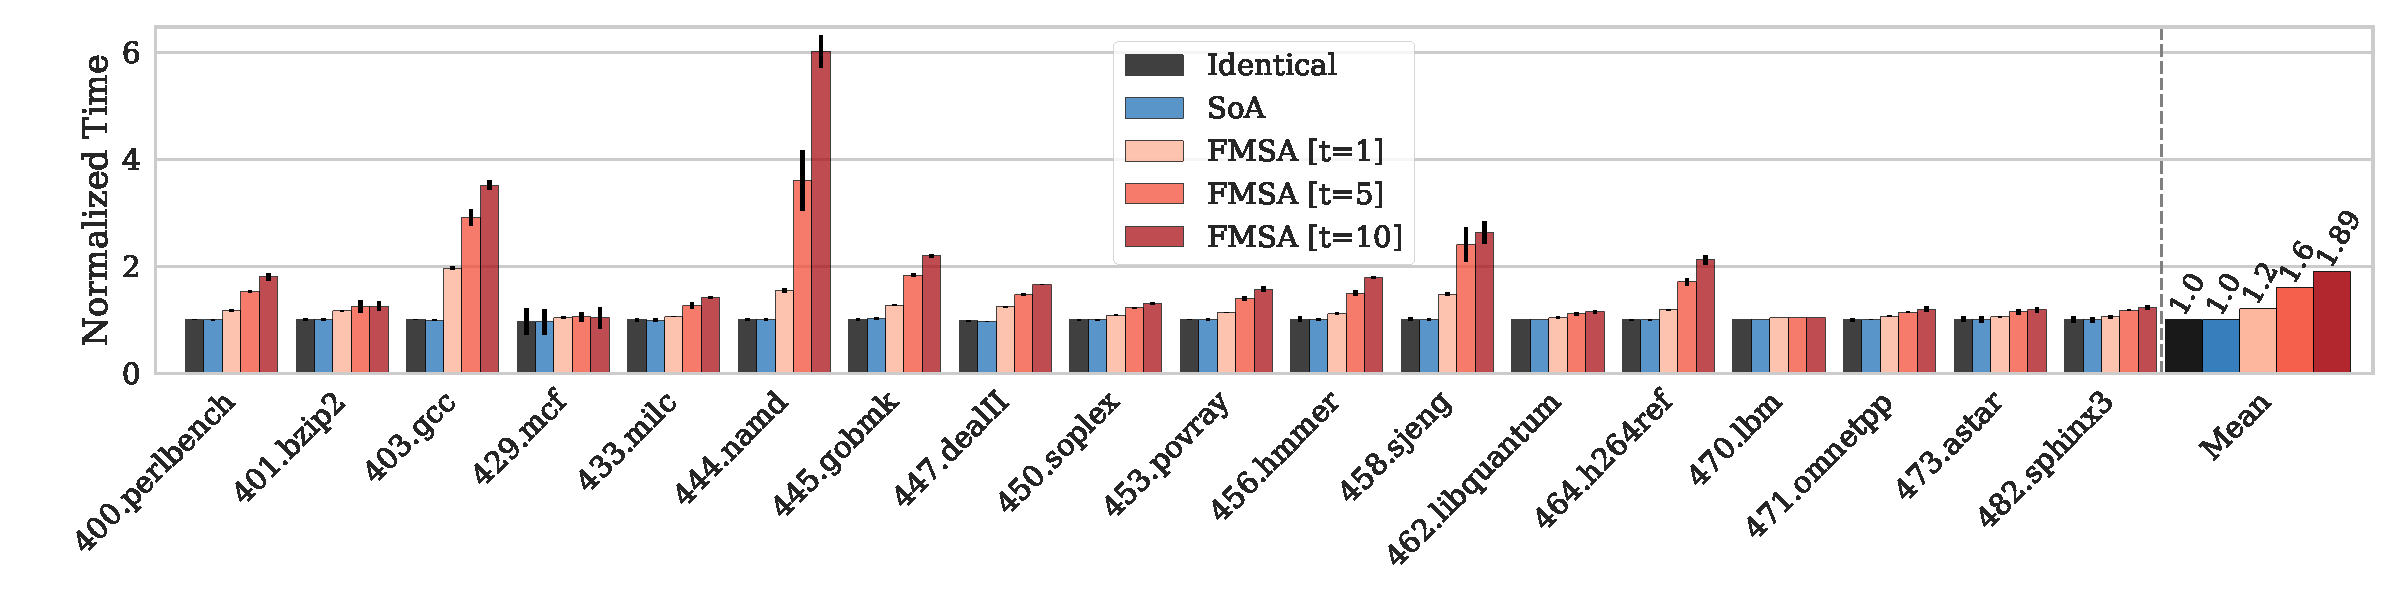
\includegraphics[width=\linewidth]{figs/compilation-time.pdf}
	\caption{Compilation-time overhead on the Intel platform. For exhaustive exploration (not shown) the average overhead is 25$\times$. Through ranking, we reduce overhead by orders of magnitude. For an exploration threshold of one, FMSA has an overhead of only 20\%.}
  \label{fig:compilation-time}
\end{figure*}

Table~\ref{tab:stats-mibench} provides more detailed statistics for MiBench.
LLVM achieves very limited results, reducing \texttt{jpeg\_c} by just 0.13\%,
\texttt{jpeg\_d} by 0.1\%, and \texttt{ghostscript} by 0.02\%, while having no effect on \texttt{typeset}.
This happens because all the functions merged by LLVM's identical technique are tiny functions relative to the overall size of the program.
Most of these functions comprise of just a few IR instructions. For example, in the \texttt{typeset} benchmark,
while it is able to merge a pair of functions, they only have five instructions. For the same benchmark, FMSA performs several merge operations, one of them between two functions with over 500 instructions.
Overall, the state-of-the-art does slightly better than LLVM's identical technique but even in its best case it cannot reduce code size more than 0.7\%.

Because these embedded benchmarks are much smaller than those in the SPEC suite, trivially similar functions are much less frequent.
This is why neither the state-of-the-art nor LLVM's identical function merging technique had any real effect on these benchmarks.
Our technique can look beyond trivially similar functions which allowed it to achieve significant code size reduction on these real embedded benchmarks.

\subsection{Compilation Overhead}

Figure~\ref{fig:compilation-time} shows the compilation-time overhead for all optimizations. As explained in the experimental setup, we
only present results when compiling for the Intel platform. Since we cross-compile on the same machine for both targets, compilation times
are very similar. We also do not include results for the oracle (exhaustive) exploration. It would be hard to visualize it in the same plot
as the other configurations, since it can be up to 136$\times$ slower than the baseline.

Unlike the other evaluated techniques, our optimization is a prototype implementation, not yet tuned for compilation-time. We believe that
compilation-time can be further reduced with some additional engineering effort. Nevertheless, by using our ranking infrastructure to
target only the single most promising equivalent function for each function we examine, we reduce compilation-time overhead by up to two
orders of magnitude compared to the oracle. This brings the average compile-time overhead to only 20\% compared to the baseline, while
still reducing code size almost as well as the oracle. Depending on the acceptable trade-off between compilation-time overhead and code
size, the developer can change the exploration threshold to exploit more opportunities for code reduction, or to accelerate compilation.

\begin{figure}[t]
  \centering
  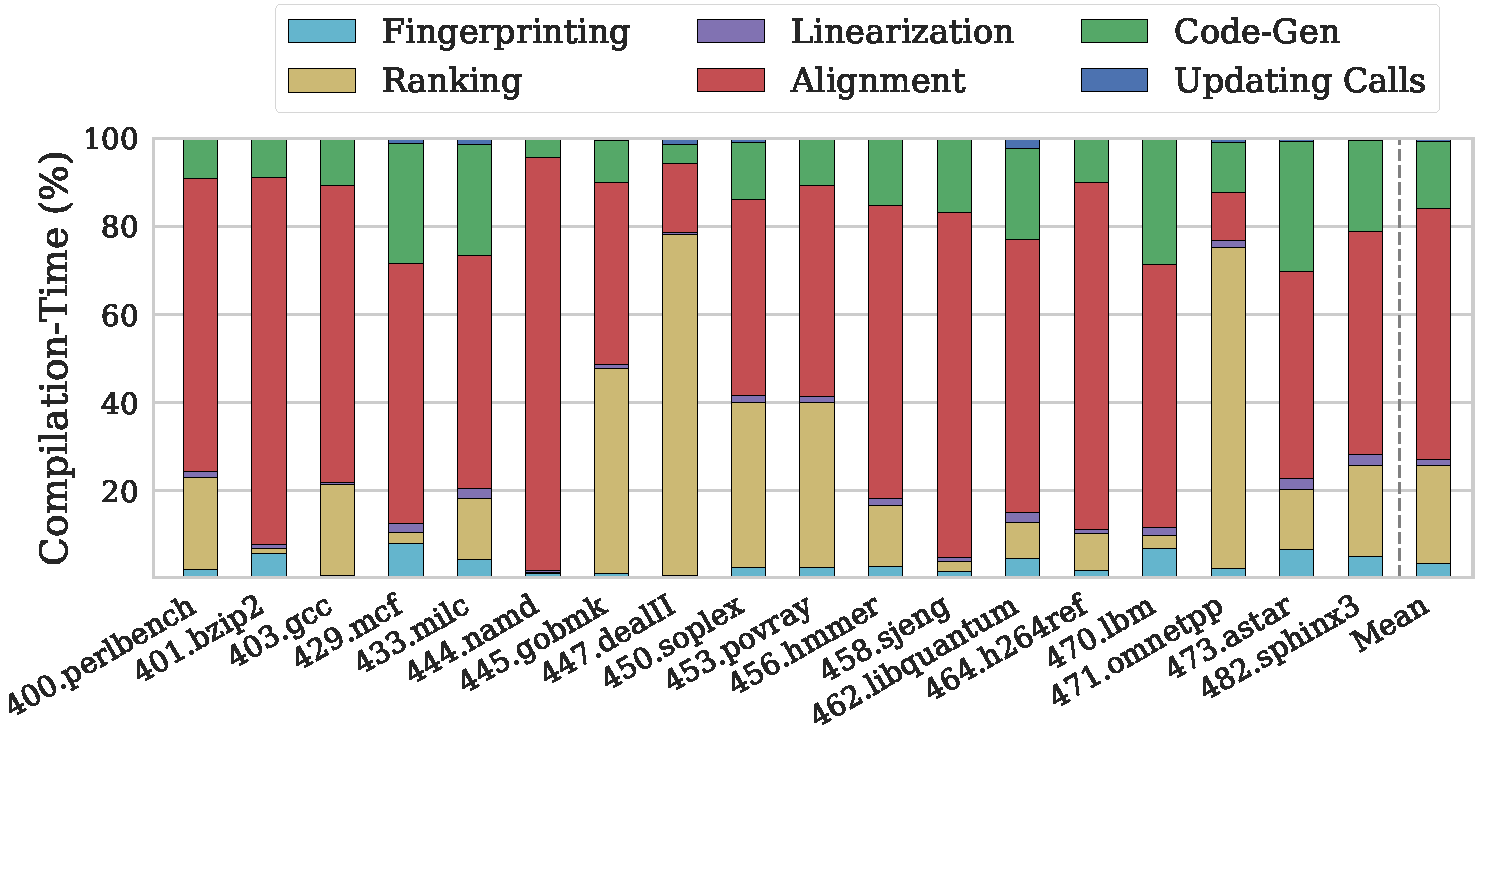
\includegraphics[width=1.0\linewidth]{figs/compilation-time-breakdown-sqrd.pdf}
  \caption{A compilation-time breakdown isolating the percentage for each major
           step of the optimization (t=1).}%, with an exploration threshold of one.}
  \label{fig:compilation-time-breakdown}
\end{figure}

\begin{figure*}[t]
  \centering
  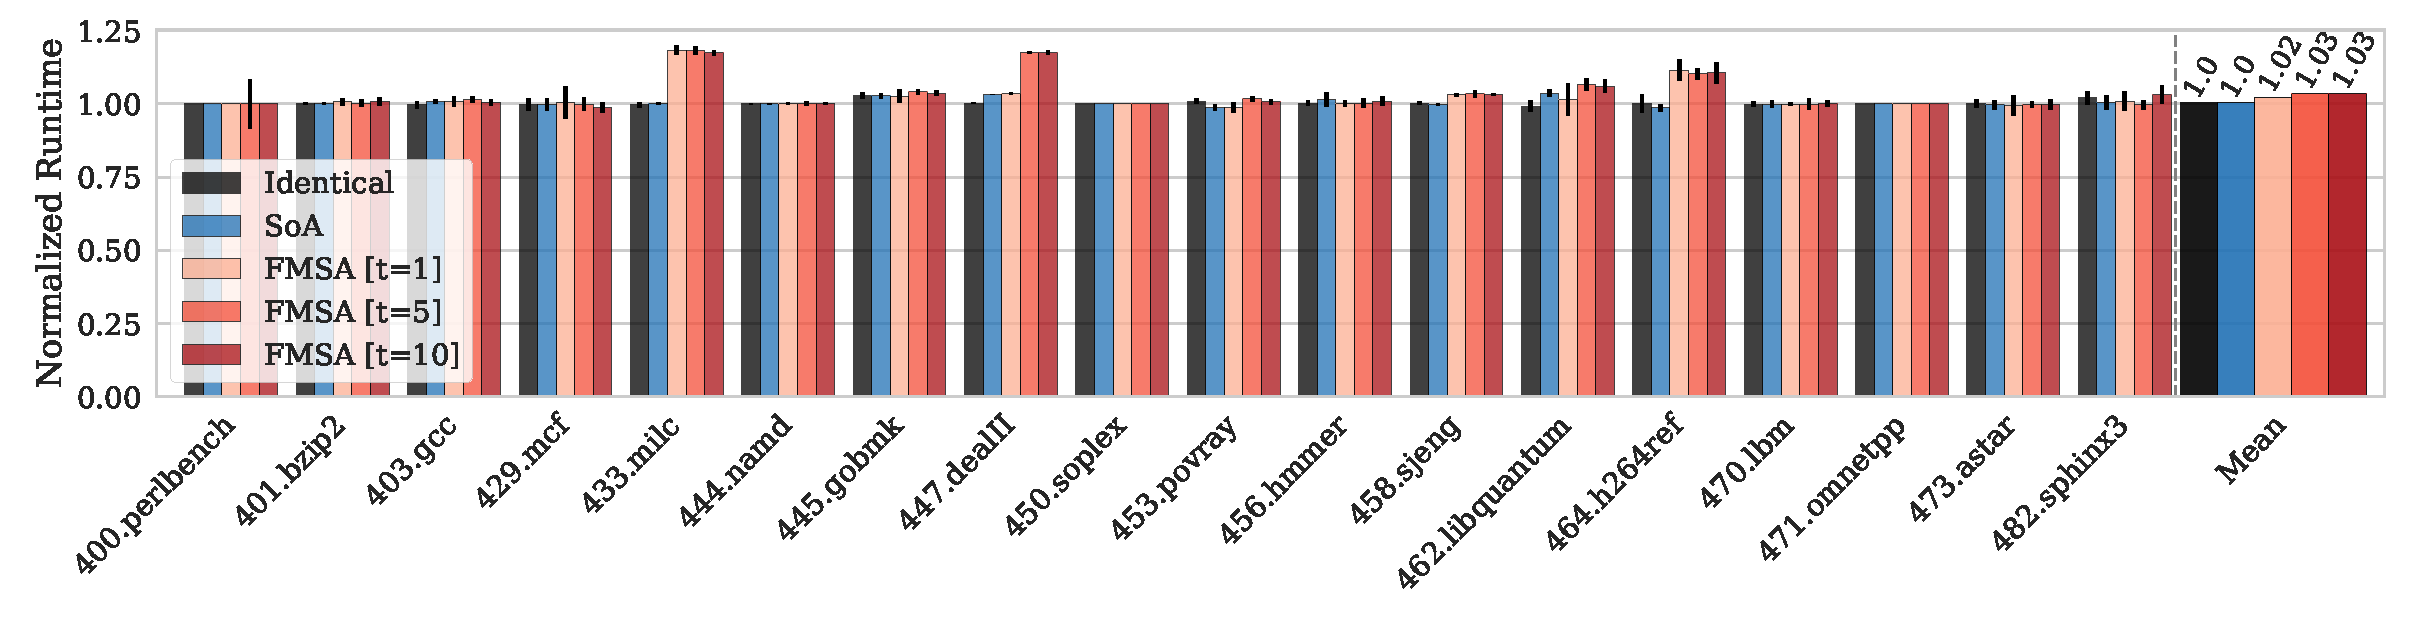
\includegraphics[width=\linewidth]{figs/runtime-impact.pdf}
  \caption{Runtime overhead on the Intel platform. Performance impact is almost always statistically insignificant. For the few benchmarks affected, FMSA merges hot functions.}
  \label{fig:runtime-impact}
\end{figure*}

Figure~\ref{fig:compilation-time-breakdown} shows a detailed compilation-time breakdown. For each major step of the proposed optimization,
we present the accumulated time spent across the whole program. To better understand the overhead of each step, we use an exploration threshold of one ($t = 1$). Because the ranking mechanism performs a quadratic operation on the number of functions, computing
the similarity between all pairs of functions, it is expected that ranking would be amongst the most costly steps. However, it is
interesting to notice that the sequence alignment dominates most of the compilation-time overhead, especially considering that this
operation is performed only once per function, when $t = 1$. Although this operation is linear in the number of functions, the
Needleman-Wunsh algorithm~\cite{needleman70} is quadratic in the size of the functions being aligned, both in time and space.
Unsurprisingly, code generation is the third most costly step, which also includes the time to optimize the merge of the parameters. The
remaining steps contribute, in total, a small percentage of all the compilation-time overhead. This analysis suggests that optimizing the
sequence alignment algorithm and the ranking mechanism is key to reducing even further the overall compilation-time overhead.

\subsection{Performance Impact}


The primary goal of function merging is to reduce code size. Nevertheless, it is also important to understand its impact on the programs'
execution time and the trade-offs between performance and code size reduction. Figure~\ref{fig:runtime-impact} shows the normalized
execution time. Overall, our optimization has an average impact of about 3\% on programs' runtime. For most benchmarks, there is no
statistically significant difference between the baseline and the optimized binary. Only for \texttt{433.milc}, \texttt{447.dealII}, and
\texttt{464.h264ref} there is a noticeable performance impact.



%\begin{figure}[t]
%  \centering
%  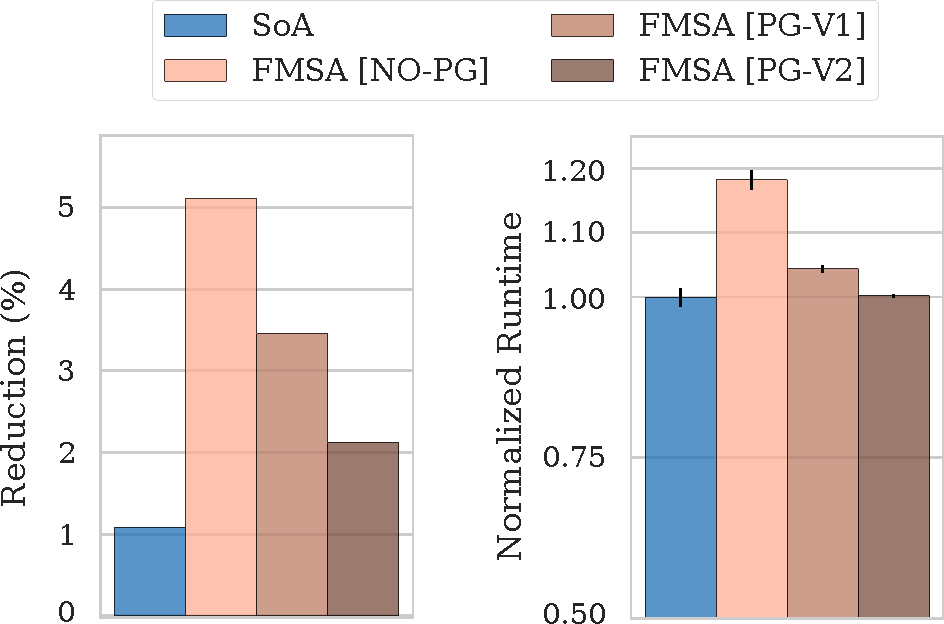
\includegraphics[width=0.8\linewidth]{figs/profiling-results.pdf}
%  \caption{Profile-guided function merging on the \texttt{433.milc} benchmark.}
%  \label{fig:pgo-results}
%\end{figure}

We take \texttt{433.milc}, which has the worst result, for discussion. For an exploration threshold value of one, we merge 58 functions.
Through profiling, we discovered that a handful of them contain hot code, that is, they have basic blocks that are frequently executed. If we prevent these hot
functions from merging, all performance impact is removed while still reducing code size. Specifically, our original results showed a
5.11\% code size reduction and an 18\% performance overhead.
Avoiding merging hot functions results in effectively non-existent performance impact and
a code size reduction of 2.09\%.
This code size reduction is still about twice as good as the state-of-the-art. As with the
compilation overhead, this is a trade-off that the developer can control.

%Note that the state-of-the-art has a reduction of only 1.09\% on this benchmark.
%If we can be more permissive, allowing some of the hot functions to be merged,
%we can have a code size reduction of 3.43\% while keeping the performance impact
%at about 4\%.

%However, \text{quantum\_gate1} is the largest function in the program,
%which means that this merge operation greatly contributes
%to the overall code-size reduction.
%Preventing this merge results in the code-size reduction dropping from 16\% to
%6.9\%, which is still a very significant code-size reduction compared to the
%other techniques that show no reduction on this particular benchmark.

%It is interesting to note that, for the 447.dealII benchmark, FMSA [t=1] has
%no extra impact than the state-of-the-art


%As a case study, we analyze the performance impact on the \text{462.libquantum}
%benchmark.
%After a detailed inspection of the program's execution with profiling
%information, we identified only two functions that contain the hottest basic
%blocks in the whole program.
%Hot basic blocks are determined based on the block frequencies recorded by
%instrumenting all basic blocks in the program~\cite{ball94}.
%The two hottest functions are: \text{quantum\_gate1} and
%\text{quantum\_decohere}.
%If we cross this information with the list of merged functions, we can confirm
%that the function \text{quantum\_gate1} is involved in a merge operation with
%a non-identical function.

%If, instead, we prevent this function of being merged, the performance
%impact goes away and we end up with a performance which is statistically
%equivalent to the baseline version.
%However, \text{quantum\_gate1} is the largest function in the program,
%which means that this merge operation greatly contributes
%to the overall code-size reduction.
%Preventing this merge results in the code-size reduction dropping from 16\% to
%6.9\%, which is still a very significant code-size reduction compared to the
%other techniques that show no reduction on this particular benchmark.
